%% -*- coding: utf-8 -*-
\documentclass[12pt,pagesize,paper=landscape,paper=192mm:108mm]{scrbook}
% 1920x1080 1280x720
\areaset[current]{192mm}{108mm}
\usepackage[T2A]{fontenc}
\usepackage[utf8]{inputenc}
\usepackage[english,russian]{babel}
\usepackage{microtype}
\usepackage{misccorr}
\usepackage{cmap}
%\usepackage[unicode=true]{hyperref}
\usepackage{graphicx}
\usepackage{amssymb}
\usepackage{amsmath}
%\usepackage{srcltx}
\usepackage{textcomp}
\usepackage{xspace}
%научные символы и смайлики \smiley \frownie
\usepackage{wasysym}
\usepackage{ccicons}
\usepackage{url}
\DeclareMathOperator{\Tr}{Tr}
%перенос формул в тексте
\newcommand*{\hm}[1]{#1\nobreak\discretionary{}%
  {\hbox{$\mathsurround=0pt #1$}}{}}
\renewcommand{\epsilon}{\varepsilon}

\begin{document}
\begin{titlepage}
  \vspace*{-0.5em}
  \begin{center}    
    % \hspace*{1.5em}
    % \begin{minipage}[t]{3em}
    %   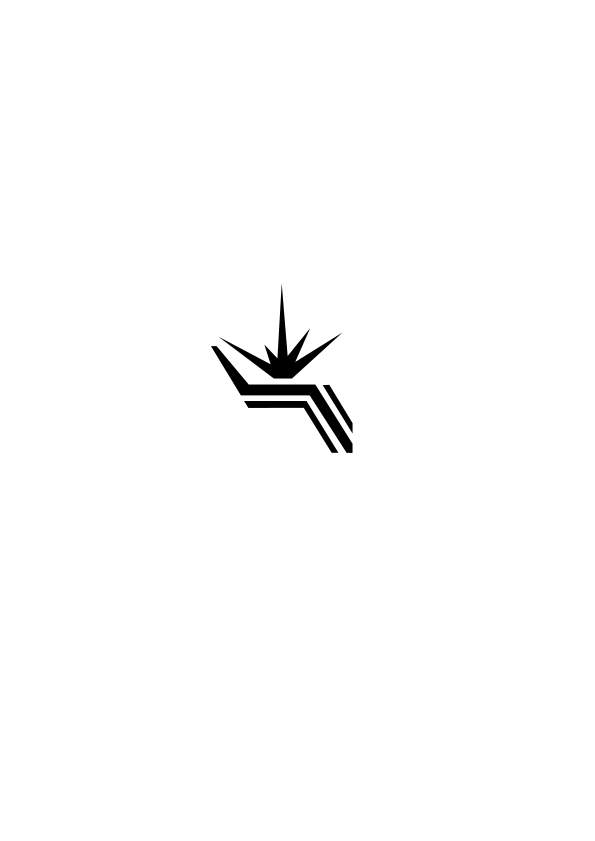
\includegraphics[width=\textwidth]{../BINP-logo}
    % \end{minipage}\hfill
    % \begin{minipage}{0.115\linewidth}
    % 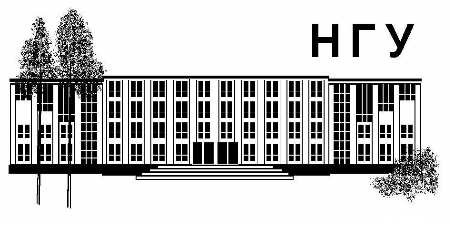
\includegraphics[width=\textwidth]{../NSU-logo}
    % \end{minipage}
    % \hfill
    % \hspace*{4.5em}
    % \smallskip

    % Кафедра физики элементарных частиц физического факультета НГУ

    % \Large
    % Профессор Андрей Грабовский
    

    % \huge
    % \textbf{Квантовая хромодинамика}

    % \Large
    % Лекция № 27
    % \vfill

    % \small
    \normalsize
    \begin{minipage}{0.75\linewidth}
      Конфигурации, для которых амплитуды туннельного перехода между
      классическими вакуумами с разными топологическими числами
      максимальны. Самодуальные и антисамодуальные поля в
      пространствах Минковского и Евклида. Инстантоны и антиинстантоны
      как решения классических уравнений движения в евклидовом
      пространстве и поля, максимизирующие амплитуды туннельного
      перехода между вакуумами с различными топологическими числами.
      $\theta$"=вакуум как состояние инвариантное относительно больших
      и малых калибровочных преобразований. Связь действия
      Янга"--~Миллса с $\theta$"=членом в вакууме с $\theta=0$ и
      действия Янга"--~Миллса без $\theta$"=члена в вакууме с~$\theta\ne0$. Появление $\theta$"=члена в лагранжиане за счет
      аксиальной аномалии при переводе кварков в массовый
      базис. Выражение аргумента определителя массовой матрицы,
      полученной при взаимодействии с полем Хиггса через фазы
      диагонализующих матриц. Выражение дипольного электрического
      момента нейтрона через параметр $\theta$. Оценка $\theta$ по
      экспериментальному пределу для~электрического дипольного момента
      нейтрона.
    \end{minipage}
    \vfill

    \normalsize \ccbysa\hspace{0.5em}  Новосибирск 2024
  \end{center}
\end{titlepage}
\end{document}

%%% Local Variables:
%%% mode: latex
%%% TeX-master: t
%%% End:
